% !TEX root = main.tex
\chapter{Simulation}
\label{chap:simulations}

  The simulation will run in several parts. First, the wings relative placement between each other will be optimized in a 2-dimensional environment. This involves, $x$- and $y$-distance between the multi-element wings, angle of attack and height relative to the chassis to give a good estimate of the wings placement range. Secondly, a 3-dimensional analysis of the entire wing with endplates will be performed. Endplate dimensions will be optimized, and further optimization of the height relative to the entire chassis to finalize the design and placement.

\section{Star-CCM+}
  Star-CCM+ was used to run the simulations of the wing first in the windtunnel for verification and next on a model of the full size wing to produce an estimate of the performance at full scale. As meshing and running the simulations were heavy computational tasks, the computations were run on the \emph{Niflheim Linux cluster supercomputer}, which is installed at the Department of Physics at DTU.

  The program numerically solves the Navier-Stokes equations, which are derived by the conservation of energy, mass and momentum through a volumetric flow. As Star-CCM+ uses the finite volume method, the equations are discretized to the conservative form: The in- and outgoing flux through a control volume must be conserved. Mathematically, this is expressed as:

  \begin{align}
    \frac{\delta}{\delta t} \iiint Q dV + \iint F dA = 0
  \end{align}
  Where $Q$ is the vector of the conserved variables (eg. $\rho =$ density), $F$ is the vector of fluxes(eg. $\rho u =$ mass flux, $\rho u^2 + p=$ momentum flux + pressure force) and $V$ is the control volume element and $A$is the surface area of the control volume element. The turbulence model Star-CCM+ employs is a K-epsilon turbulence model which is the most commonly used in computational fluid dynamics. %The equations Star-CCM+ solves are the turbulent kinetic energy $k$:
  %\begin{align}
  %  \frac{\delta (\rho k)}{\delta t} + \frac{\delta (\rho k u_i)}{\delta x_i} &= \frac{\delta}{\delta x_j} \left(\frac{\mu_t}{\sigma_k}\frac{\delta k)}{\delta x_j}\right) + 2\mu_t E_{ij}E_{ij}-\rho \epsilon
  %  \intertext{and the dissipation $\epsilon$:}
  %  \frac{\delta (\rho \epsilon)}{\delta t} + \frac{\delta (\rho \epsilon u_i)}{\delta x_i} &= \frac{\delta}{\delta x_j} \left(\frac{\mu_t}{\sigma_\epsilon}\frac{\delta \epsilon)}{\delta x_j}\right) + C_{1\epsilon} \frac{\epsilon}{k} 2\mu_t E_{ij}E_{ij}-C_{2\epsilon}\rho \frac{\epsilon^2}{k}
  %\end{align}

  The interested reader of how Star-CCM+ works is referred to the \emph{User Guide Star-CCM+, version 13.02}.

\section{Mesh Generation}
\label{sec:mesh}
  The mesh has to be structured in accordance to best practice. Areas with high velocity and pressure gradiants have to be dissolved in acceptable resolutions, in order to ensure correct results. Running an initial test on a generic mesh made it clear where the volumemesh requires greater resolution. Gradiants are easily visible around the wing's leading edge, and generally around the solid bodies. Furthermore, aligning the mesh with the flow improves accuracy and rate of convergence. To determine the convergence of simulation results six different mesh resolutions where used to examine the simulations for the windtunnel setup with a wind velocity of $\SI{40}{\metre\per\second}$. Finding the minimum mesh resolution where results have converged with higer resolution results, means a minimum computation time can be achived and thereby allowing for more simulations to be run.

  \begin{figure}
    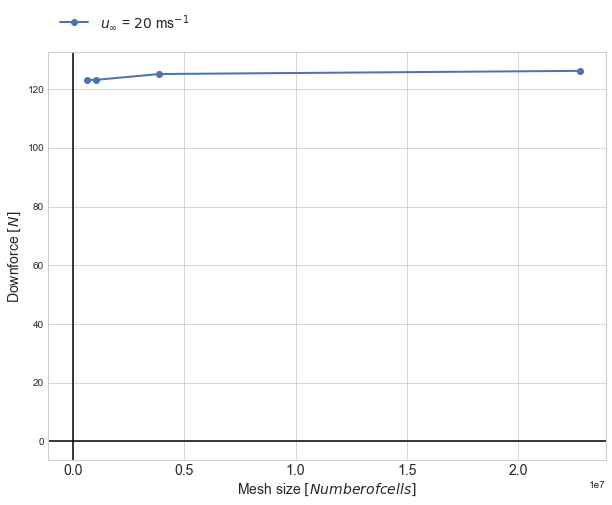
\includegraphics[width=\textwidth]{DFprmeshsize}
    \caption{Normalized downforce as a function of mesh size. Plotted to see the convergence towards the same force.}
    \label{fig:DFprmeshsize}
  \end{figure}

  Generating a mesh of correct size is done by sampling downforce over a range of mesh sizes. In figure \ref{fig:DFprmeshsize}, the normalized downforce is plotted as a function of the mesh size. The mesh independence study shows that the function converges to acceptable levels near the mesh size $\SI{.4E7}{}$, and serves to be a good compromise between results and computing time.

\section{Optimizing the Rear Wing}

  As mentioned in chapter \ref{chap:conceptdesign}, there's a large variation in parameters to optimize for. Numerical optimization has been done on end plates size and relative position of the two wing elements.


  \subsection{Verification of Simulation Results}
  \label{sec:simulationcomparison}

  The data from the experimental test with the $\frac{1}{4}$ scale was first plotted to obtain a picture of the surface pressure on the test wing. An example of a mean over 3000 pressure readouts for a wind speed of $\SI{40}{\metre\per\second}$ is shown in figure \ref{fig:surfacepressureint}, with the standard deviation shown as errorbars. Measurements were run in wind tunnel from $\SI{10}{\metre\per\second}$ to $\SI{60}{\metre\per\second}$ in steps of $\SI{10}{\metre\per\second}$.

  \begin{figure}
    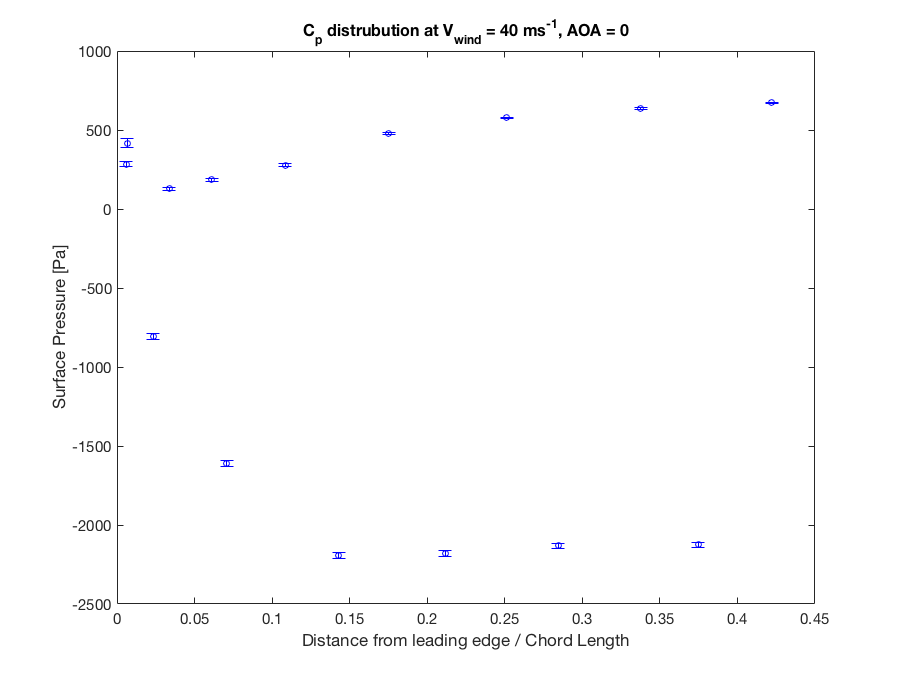
\includegraphics[width=\textwidth]{surfacepressureint}
    \caption{Surface pressure readout from the 15 pressure taps at wind speed $\SI{40}{\metre\per\second}$ in the wind tunnel. Pressure readout is meaned over 3000 measurements and shown with errorbars representing the standard deviation of the measurements.}
    \label{fig:surfacepressureint}
  \end{figure}

  Simulations were then run in \emph{Star-CCM+}. Firstly the CAD model of the $\frac{1}{4}$-scaled wing was imported in the software, then the dimensions of the Red wind tunnel was drawn and the CAD model was placed in the same location as in the real tunnel test. The setup was then volume mesheded with a cell count of around $0.4 \cdot 10^{7}$ million cells as found in section \ref{sec:mesh}. A 2D view of the 3D mesh is shown in figure \ref{fig:mesh3point8mill}. After meshing the physics model for the simulation is set, and simulations are run for the different wind velocities.

  \begin{figure}
    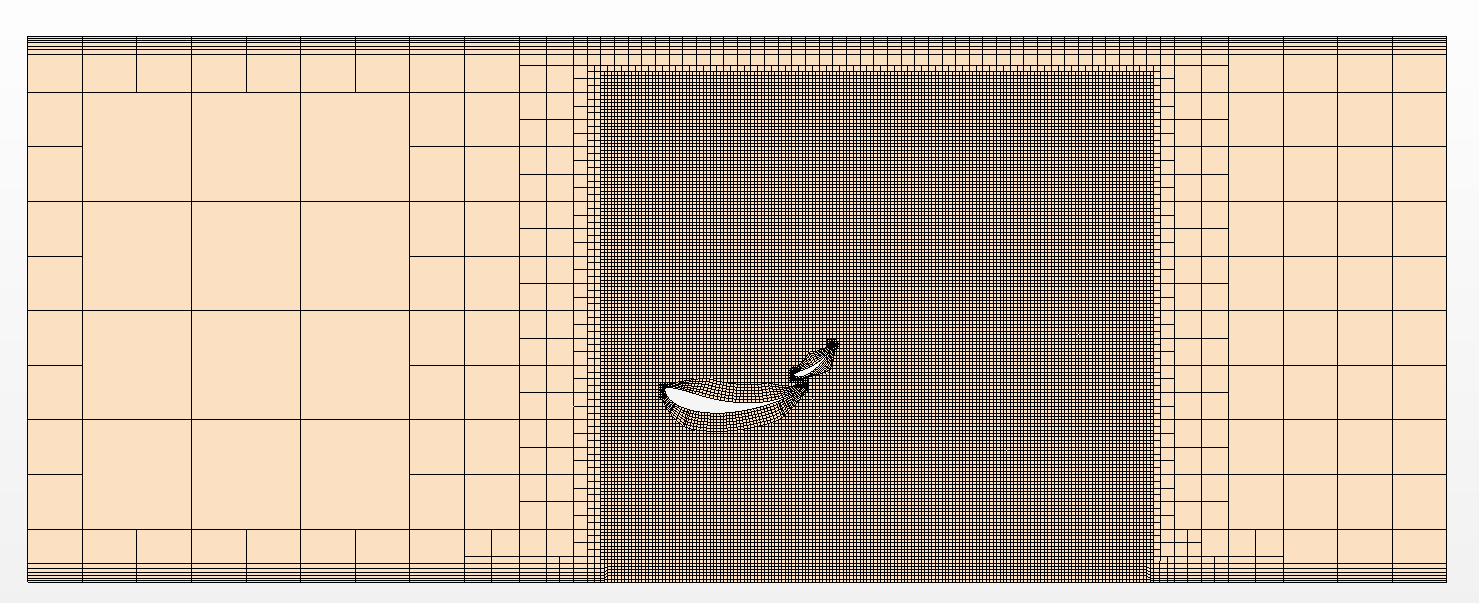
\includegraphics[width=\textwidth]{mesh3point8millcells}
    \caption{2D cut through of the 3D mesh used for simulations of the wind tunnel test.}
    \label{fig:mesh3point8mill}
  \end{figure}

  The simulations are run until the simulation reseults converges to a result. Monitors of the dragforce and downforce for the wing found by the simulation were used to the convergence of the results, an example is shown in figure \ref{fig:downforcemonitor}. Furthermore scalar views and vector views of the pressure distribution and wind velocity around the wing profile can visually help verify that the solutions does not have any obvious faults, such as areas with extremly high velocity og pressure indicating the solutions is not realistic. Examples of a scalar view for the pressure distribution and a vector view of the wind velocity are shown in \ref{fig:pressureScalarV40} and \ref{fig:velocityScalarV40}.

  \begin{figure}
    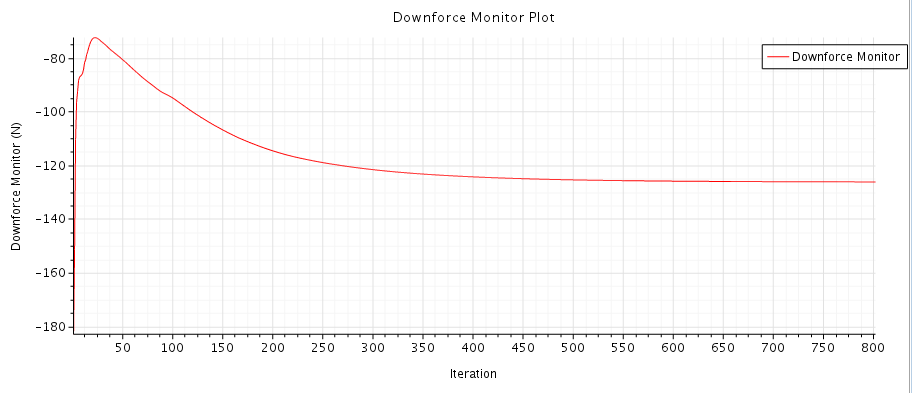
\includegraphics[width=\textwidth]{downforcemonitor}
    \caption{Monitor of the convergence of the downforce over the number of iterations in Star-CCM+, here shown for a wind velocity of $\SI{40}{\metre\per\second}$.}
    \label{fig:downforcemonitor}
  \end{figure}

  \begin{figure}
    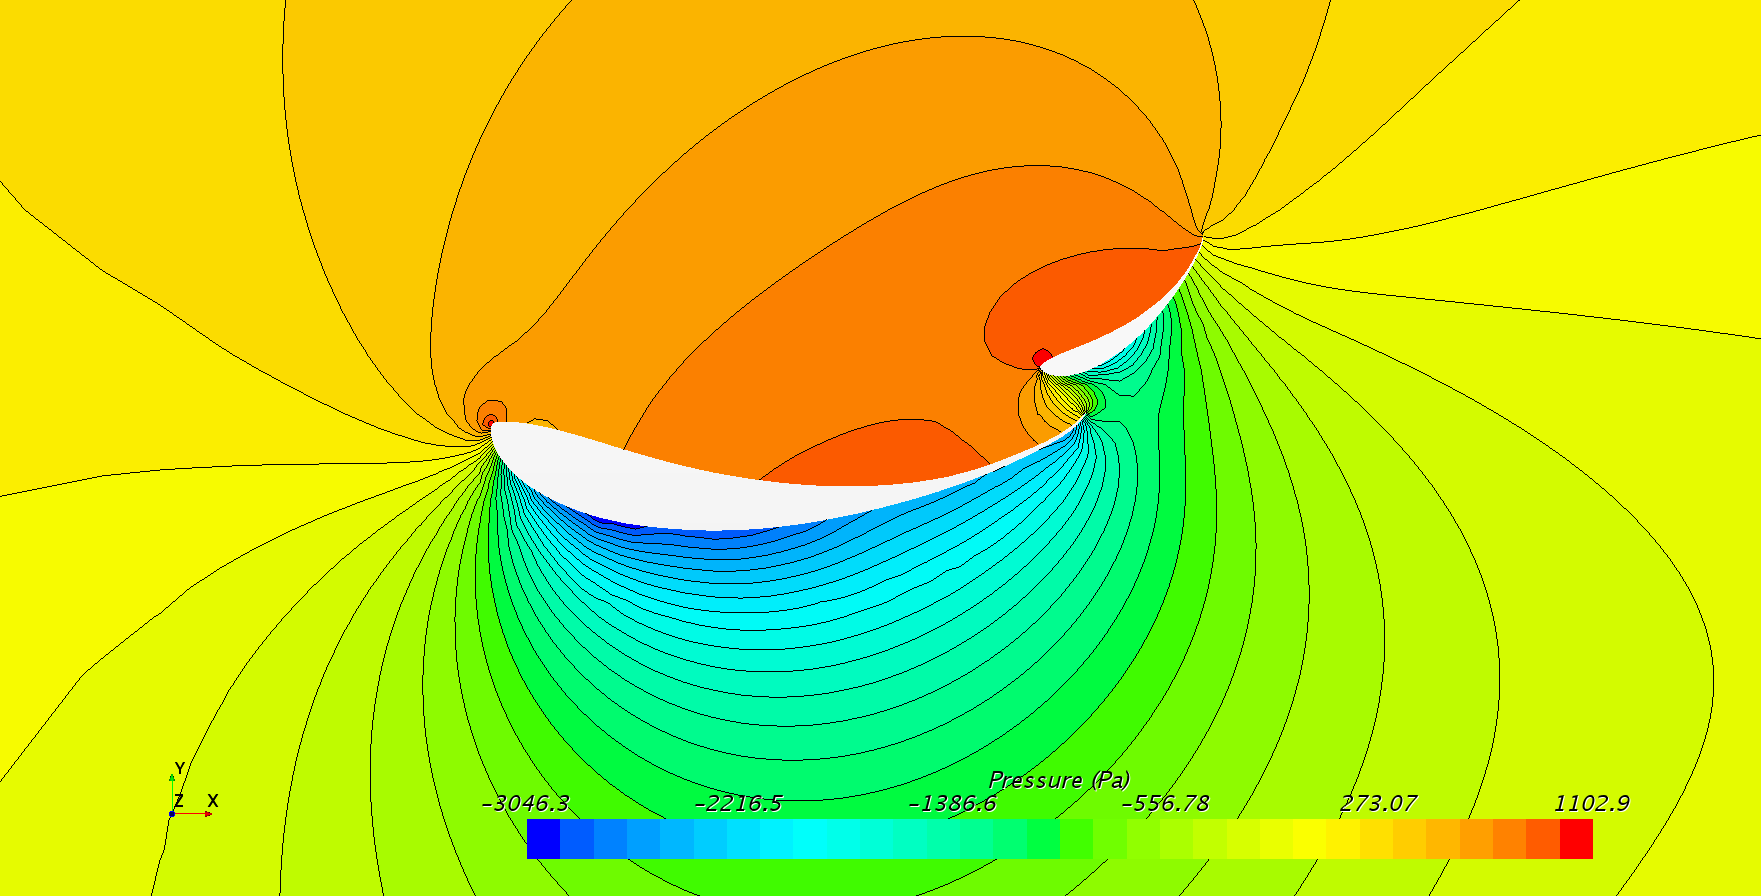
\includegraphics[width=\textwidth]{pressureScalarV40}
    \caption{Scalar view of the pressure distribution surrounding the two elements of the wing, here at a wind velocity of $\SI{40}{\metre\per\second}$.}
    \label{fig:pressureScalarV40}
  \end{figure}

  \begin{figure}
    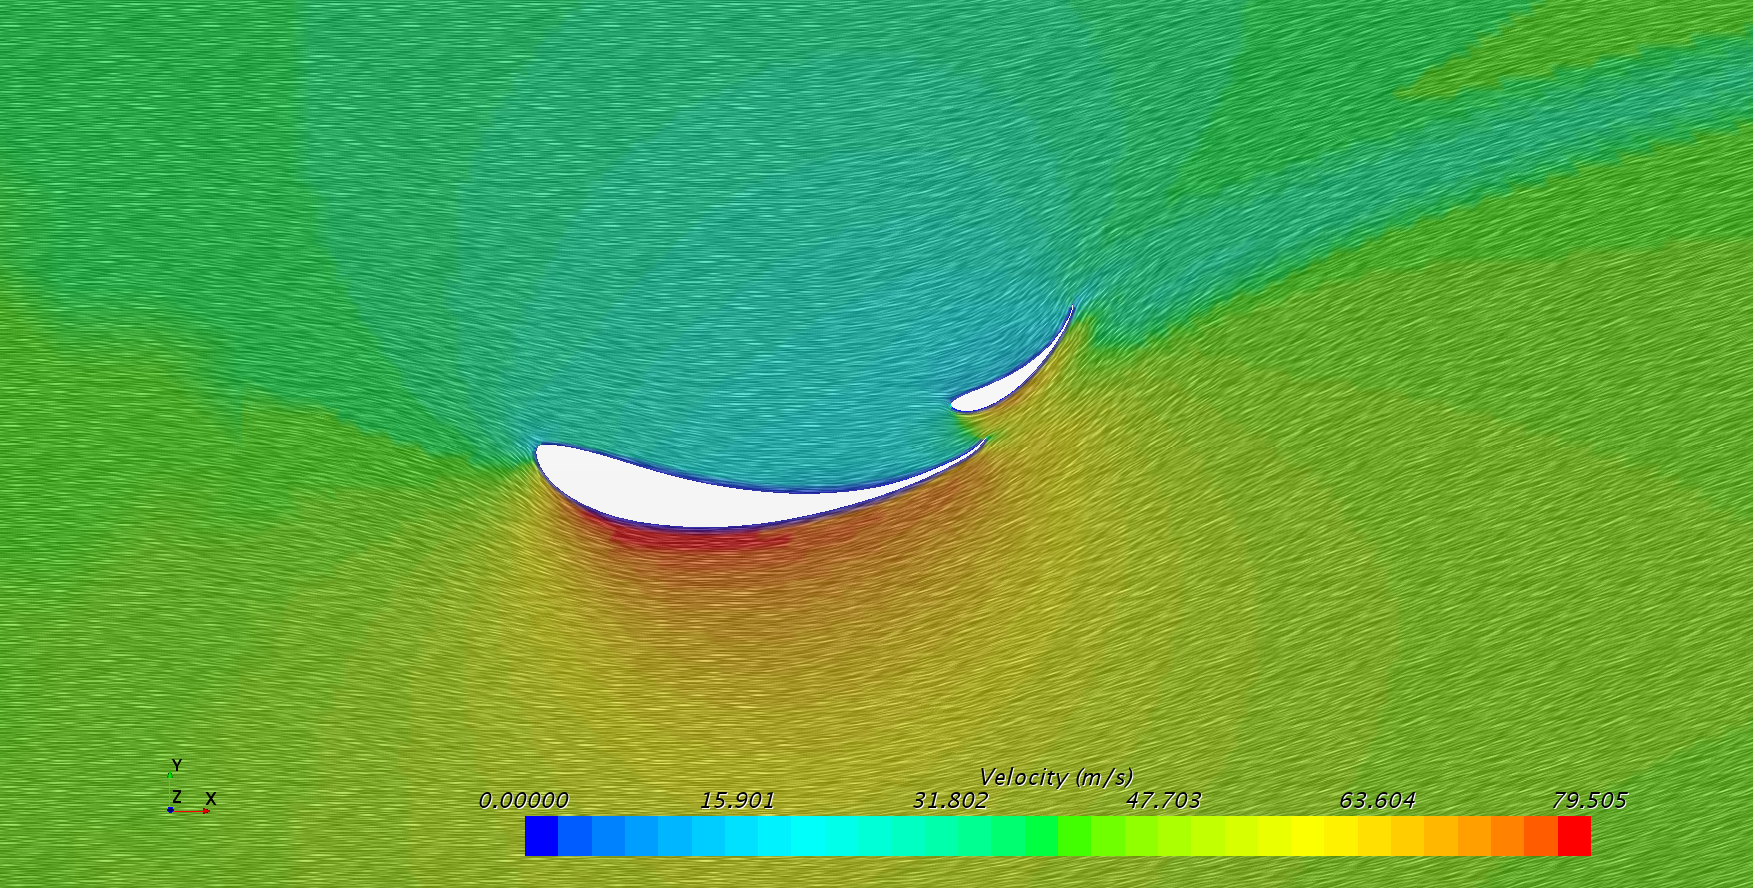
\includegraphics[width=\textwidth]{velocityScalarV40}
    \caption{Vector view of the wind velocity surrounding the wing, here at a wind velocity of $\SI{40}{\metre\per\second}$.}
    \label{fig:velocityScalarV40}
  \end{figure}

  From the simulations the surface pressure of the airfoils was also found, and saved to compare with the measurements of the surface pressure from the real wind tunnel test. The simulated surface pressure is shown in figure \ref{fig:simsurfacepressurev40}.

  \begin{figure}
    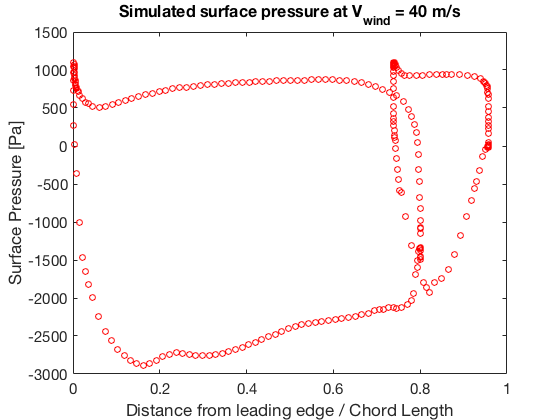
\includegraphics[width=\textwidth]{simsurfacepressurev40}
    \caption{Simulated surface pressure on both elements of the wing. To the left the larger element surface pressure and the smaller elements surface pressure is shown right. Simulated at wind velocity of $\SI{40}{\metre\per\second}$.}
    \label{fig:simsurfacepressurev40}
  \end{figure}

  Comparing the surface pressure predicted by the simulation,\ref{fig:simsurfacepressurev40}, and measured in the test, \ref{fig:surfacepressureint}, show that two are not i sync. Comparing the predicted downforce and measured downforce, shows that the simulated results predict a $\SI{40}{\%}$ downforce than measured. This could be caused by several factors. One factor could be the assembly of the test wing is not a perfect replica of the full scale wing, an improement to help this would be by producing the scaled model completely by machining with small tolerances, compared to the half machined and half handbuild model used in these test. This could cause the relative position of the 2 wing elements to be diffrent from the CAD model used in simulations.

  Finding the correct correlation between the estimated downforce and extact surface pressure will not be possible in this report. The simualtions and measurements can however be compared by using the dimensionless number, the pressure coefficient,

  \begin{align}
    C_p \equiv \frac{p-p_{\infty}}{\frac{1}{2}\rho_{\infty}V_{infty}^2},
  \end{align}

  where $p$ is the static pressure at the point being evaluated, $p_{\infty}$ is the static pressure in the freestream, $\rho_{\infty}$ is the freestream fluid density and $V_{\infty}$ is the freestream velocity of the fluid. The pressure coefficient describes the relative pressure throughout a fluid in movement. In many situations the pressure coefficient near a body is independt of the size of the body. \fixme{Consider moving to theory}

  The pressure coefficient allows us to compared the form of the relative pressure between the simulations and the experimental test. This comparison is shown in figure \ref{fig:CpV40}. When comparing the two, a difference in value is still visible due to the difference in absolute pressure, but the form of the two $C_p$ distributions, confirm the characteristics of the flow around the wing is uptain through the simulation. A higher resolution of measuring taps would help further testing, but for the smaller model is very difficult to achieve due to lack of space. \fixme{fix labels. fixed}

  \begin{figure}
    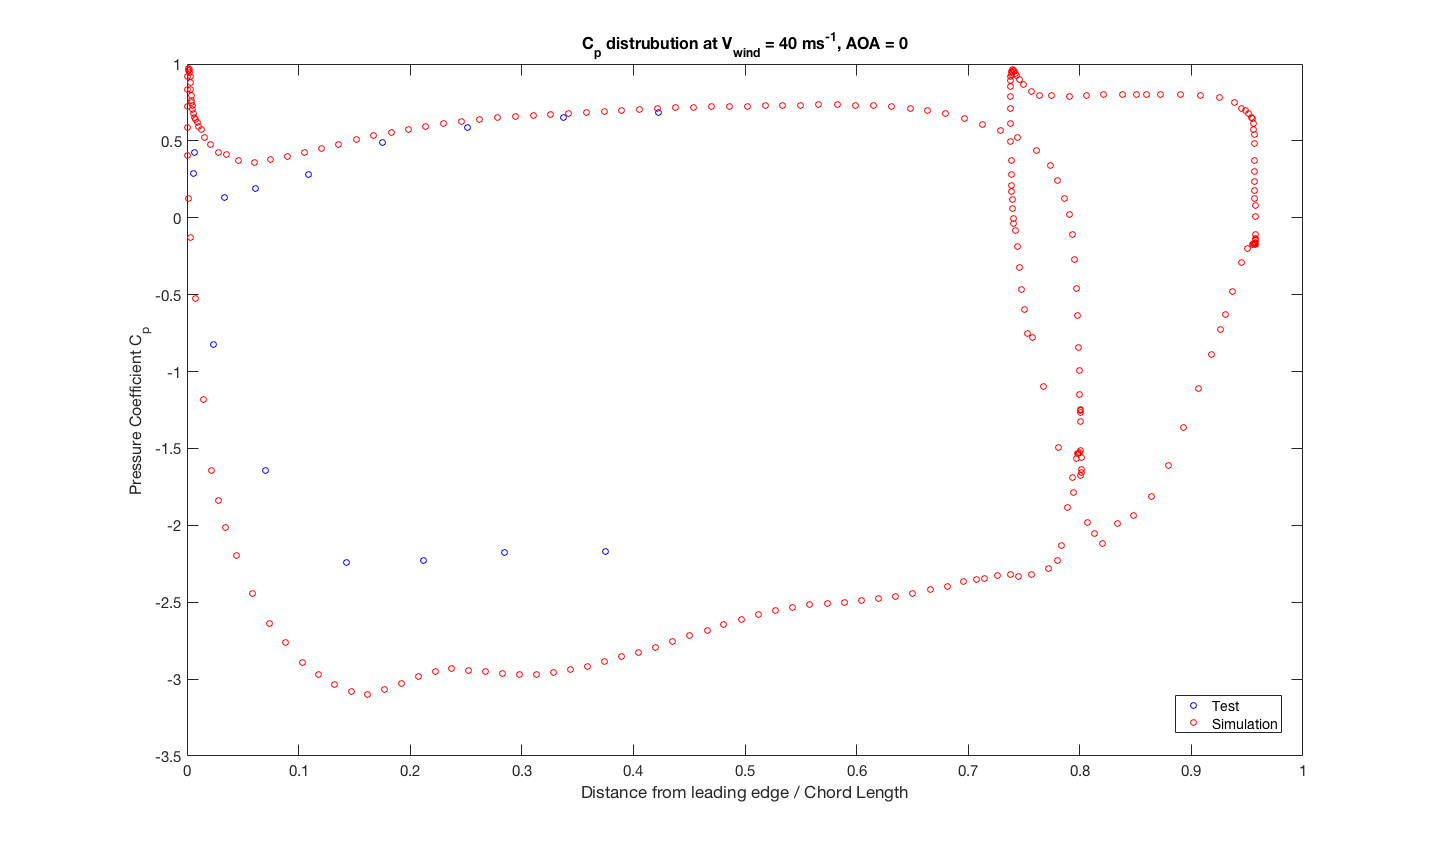
\includegraphics[width=\textwidth]{CpV40}
    \caption{Comparison of simulated and test found $C_p$ values at a wind velocity of $\SI{40}{\metre\per\second}$.}
    \label{fig:CpV40}
  \end{figure}

  The use of simulations for designing an aerodynamic package for the race car for the moment is usefull as a way to insure the realtive pressure distrubtion aorund the wing is as wanted, and ensuring that the flow does not seperate at unwanted locations. However further work on the correlation between simulated downforce and measured downforce is still needed and the work will continue with the Vermilion Racing team, in order to have the best possibilities to design a good aero-package before having to build it.

  Lastly worth noting is when the simulated flow is visualized by streamlines, the vortex generation at the rear of the wing, as mentioned in section \ref{subsec:endplates}, is shown clearly in figure \ref{fig:simvortex}. It is clear that the size of the produced vortices are interacting with the side walls of the wind tunnel. A sugestion for further testing of an wing with such large vortex generation would be to use a wind tunnel with a larger cross-secton to avoid interactions with the side walls.

  \begin{figure}
    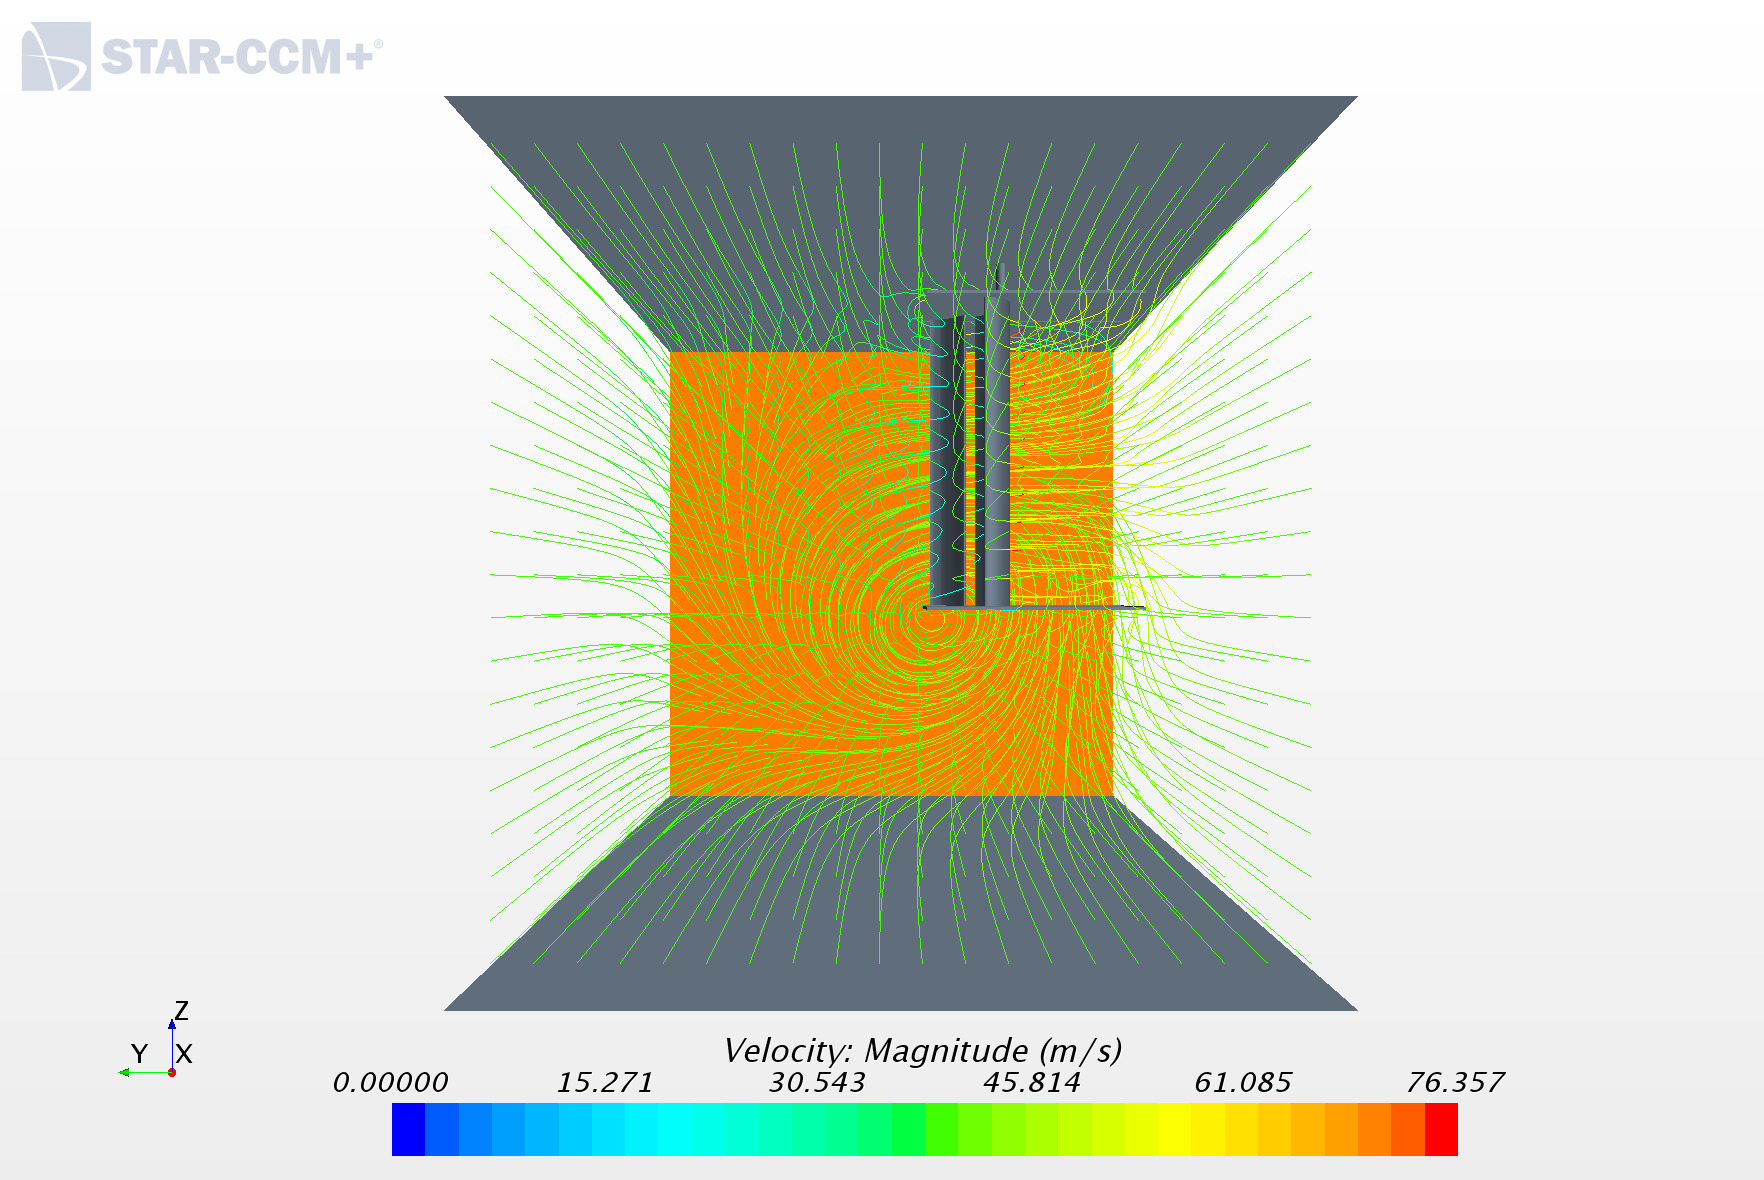
\includegraphics[width=\textwidth]{simulatedvortex}
    \caption{Visualization by streamlines of the simulated airflow around the wing. Vortex generation at the rear of the wing is visiable.}
    \label{fig:simvortex}
  \end{figure}

  \subsection{Multi-Element Wing Optimization}
  The influence of the two wing elements relative position on lift was examined to optimize the downforce the rear wing provides to the car at a given velocity. This relative position optimization was performed in the software package \emph{MultiElements Airfoils} provided from \emph{Hanley Innovations}. A scatterplot of the relative position is seen in figure \ref{fig:multieleoptimization}. The trailing edge of the first element is seem as the dark lines, and the position of the second elements leading edge is plotted, where the resulting lift coefficient is embedded as color. The redder the better lift coefficient. After sweeping, a maximum lift of $C_L = 2.60$  at $u = \SI{15}{\metre\per\second}$. is found with the leading edge of the secondary element placed at $x=\SI{0.5}{\metre},y=\SI{-0.01}{\metre}$ relative to the leading edge of the main element.

  \begin{figure}
    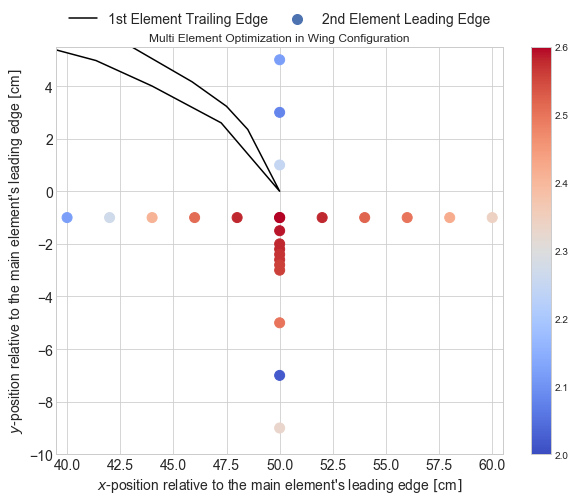
\includegraphics[width=\textwidth]{multieleoptimization2}
    \caption{Optimization of the two element wing. The redder the dots, the higher the lift coefficient.}
    \label{fig:multieleoptimization}
  \end{figure}

\section{Downforce Estimate of Full Scale Wing}
\fixme{Maybe save for defense}
